\section{The first moment}
In this section we will be interested into the first moment tensor appearing in \ref{eq:homo_momentum_c}, namely the average of the tensor $\textbf{D}_\alpha = \int_{S_\alpha} \textbf{r}\textbf{T}_c\cdot \textbf{n}_c dS = \int_{S_\alpha} \textbf{rf}_c dS$, where we introduced the microscopic hydrodynamical force vector $\textbf{f}_c = \textbf{T}_c\cdot \textbf{n}_c$.
Following the same approach as the analysis of \citet[chapter 2]{kim2013microhydrodynamics} we decompose the first moment tensor into two distinct tensors and remove the isotropic part of $\textbf{D}_\alpha$, yieldings
\begin{equation*}
    \textbf{D}_\alpha - \frac{1}{3}(\textbf{I}:\textbf{D}_\alpha)\textbf{I}
    = \textbf{S}_\alpha+\textbf{T}_\alpha,
\end{equation*}
where $\textbf{S}_\alpha$ is the stresslet tensor and $\textbf{T}_\alpha$ the hydrodynamical torque acting on the particle. 
Besides, because of numerical limitations, we prefer to use the force defined inside the dispersed phase $\textbf{f}_d$ instead of original force, $\textbf{f}_c$. 
It is possible to switch from a force to another by making use of the jumps condition (\ref{eq:stressjump}) defined in \ref{chap:avg}, i.e. $\textbf{f}_c = \textbf{f}_I - \textbf{f}_d$. 
Consequently, we can write that $\textbf{D}_\alpha = \textbf{D}_\alpha^I + \textbf{D}_\alpha^h$, where $\textbf{D}_\alpha^h$ is the hydrodynamical contribution to the first moment and $\textbf{D}_\alpha^I$ the surface tension force contribution. 
Applying the same decomposition for the torque and stresslet tensors yields,
\begin{align*}
    \textbf{S}_\alpha^h &= 
    \frac{1}{2}\int_{S_\alpha}
    \left(
        \textbf{r} \textbf{f}_d + \textbf{f}_d \textbf{r}
    \right)dS
    - \frac{1}{3}\int_{S_\alpha}
        (\textbf{r} \cdot \textbf{f}_d )\textbf{I}
        dS,\\
        \textbf{T}_\alpha^h &= 
    \frac{1}{2}\int_{S_\alpha}
    \left(
        \textbf{r} \textbf{f}_d - \textbf{f}_d \textbf{r}
    \right)dS,
\end{align*}
where we defined $\textbf{S}_\alpha^I$ and $\textbf{T}_\alpha^I$ as the contribution of the surface tension force and $\textbf{S}_\alpha^h$ and $\textbf{T}_\alpha^h$ as the hydrodynamical contribution.

The surface tension part of the first moment, $\pnavg{\textbf{D}_\alpha^I}$, can be obtained theoretically. 
Indeed, in the limit of low \textit{Bond} numbers the droplets are in average spherical.
Therefore, it is possible to compute the integral, $\int_{S_\alpha} \textbf{r} \textbf{f}_I dS$, analytically since $\textbf{f}_I $ is solely a function of the shape.
Then, the first moment of the surface tension force turns out to have the simple expression, 
\begin{align*}
    &\pnavg{\textbf{D}_\alpha^I}
    = \frac{2V_\alpha\sigma}{D_\alpha}  \textbf{I}
    &
    \text{and} 
    &&
    \pnavg{\textbf{S}_\alpha^I}
    =\pnavg{\textbf{T}_\alpha^I}
    = 0&
\end{align*}
For a detailed derivation we refer the reader to \ref{ap:cinematic}. 
It is also possible to consider other shapes than spherical, such as oblate and spheroid particles. 
These shapes might be considered for high $Bo$ and $Ga$ flows, since the droplets' shape can be approximated as a spheroid.
Again, we encourage the reader to look at \ref{ap:cinematic} for a detailed derivation of $\textbf{D}_\alpha^I$.  

Regarding the first moment generated by hydrodynamic forces theoretical investigation are not in order for the range of parameters studied here, therefore we expose our numerical results. 
First, notice that due to the symmetry of the numerical simulations all the non-diagonal components of $\textbf{D}_\alpha$ are null.
Consequently, the only non-null components in homogeneous rising suspensions flows are the three diagonal components of $\textbf{S}_\alpha^h$.
\begin{figure}[h!]
    \centering
    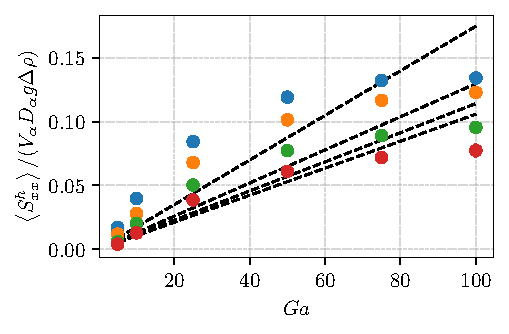
\includegraphics[height=0.3\textwidth]{image/HOMOGENEOUS/fPA/Sxx.pdf}
    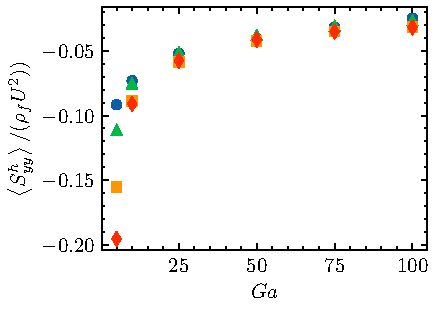
\includegraphics[height=0.3\textwidth]{image/HOMOGENEOUS/fPA/Syy.pdf}
    \caption{(left) Dimensionless trace of the first moment in terms of the \textit{Galileo} number for different $\phi$. (dots) Numerical simulations, (dashed line) empirical formula \ref{eq:trD_scaling}.
    (right) Dimensionless diagonal components of the stresslet tensor, ($\bullet$) are the vertical components, $S^\alpha_{yy}$, ($\blacktriangle$) are the horizontal components, $S^\alpha_{xx} = S^\alpha_{zz}$. (dashed line) empirical formula \ref{eq:B_scaling}.}
    \label{fig:trD_Sx_Sy}
\end{figure}
On \ref{fig:trD_Sx_Sy} we can observe that the dimensionless first moment's trace or spherical part has a quite simple tendency with the Galileo number.
Indeed, as depicted by the black dashed line in \ref{fig:trD_Sx_Sy} (left) the first moment behave in the dilute limit as a linear function with the \textit{Galileo} number, 
\begin{equation}
    \frac
    {\pnavg{\textbf{I}:\textbf{D}_\alpha^h}}
    {3V_\alpha D_\alpha g (\rho_f - \rho_d)}
    \sim  -1.44\cdot 10^{-03} Ga.
    \label{eq:trD_scaling}
\end{equation}
However, it possesses a non-monotonic behavior with respect to $\phi$. 
Determining whether the observed effect is a result of a numerical artifact or due to physical phenomenon is difficult to figure out.

On \ref{fig:trD_Sx_Sy} (right) we observe the proportion of each component of $\textbf{S}_\alpha^h$. 
Thus, we remark that the first moment gets isotropic for low $Ga$ and high $\phi$.
Then, the first moment decrease in the direction of the flow and increase on the direction perpendicular to the flow, as indicated by the ratios on the \ref{fig:trD_Sx_Sy} (right).
In conclusion, we suggest the following empirical formula for the first moment valid in the dilute regime, namely
\begin{equation}
    \pnavg{\textbf{S}^h_\alpha}
    =\frac{1}{3} \pnavg{\textbf{I}:\textbf{D}_\alpha}
    \left(
        \textbf{I} 
        + \pnavg{\textbf{B}}
    \right),
\end{equation}
where $\pnavg{\textbf{I}:\textbf{D}_\alpha}$ is defined by \ref{eq:trD_scaling} and $\pnavg{\textbf{B}}$, by,
\begin{equation}
    \pnavg{\textbf{B}} = 3.93 \cdot 10^{-04} ((\textbf{I}-\textbf{dd})-2\textbf{dd}).
    \label{eq:B_scaling}
\end{equation}
Based on this last empirical formula we observe that the stresslet is twice larger and with opposite sign in the direction of the flow than on the plan normal to the flow direction. 
In other words the mean force traction on the surface of the particle is in traction in the direction of the flow and in compression in the plan normal to the flow, besides the force traction is twice larger in the direction of the flow. 